\section{RAVEN Concepts}
\label{sec:RAVENconcept}
After the brief overview of the RAVEN inside structure, we can illustrate how this translates into capabilities and how the user can access them.

\begin{itemize}
    \item \textit{RAVEN entities}: Section ~\ref{sub:EntitiesAndFlow} is aimed to provide an overview on how the different objects in
    RAVEN can interact with each other, generating the user-dependent analysis flow;
    \item \textit{RAVEN input main components}: Section ~\ref{sub:InputStructure} provides a brief introduction of the input structure, introducing
    some of the input ``structure'' that are going to be used in this manual. A detailed explanation of the
    input structure and keywords is reported in the user manual ~\cite{RAVENuserManual}.
\end{itemize}

\subsection{RAVEN entities and analysis flow}
\label{sub:EntitiesAndFlow}
In the RAVEN code, the the number of analyses that can be performed is virtually ``infinite'',
since the code is modular and object oriented.
In the RAVEN code the number and types of possible analyses is potentially large (it is customization to many problem types).
\\Each basic action (e.g. sampling, printing, etc.) is encapsulated in
a dedicated object (named ``\textbf{Entity}''). Each object is inactive till it is connected with
other objects in order to perform a more complex process. For example,
the \textit{Sampler} entity, aimed to employ a perturbation action, becomes active only in case
it gets associated with a \textit{Model}, that is the internal representation of a physical model (e.g. a system code).
\\RAVEN provides support for several \textbf{Entities}, which branch in several different categories/algorithms:
\begin{itemize}
  \item \textit{\textbf{RunInfo}}:
    \\The RunInfo \textbf{Entity} represents the container of the information regarding how the overall computation should
      be performed. This \textbf{Entity}  accepts several input settings that define how to drive the calculation and set up,
      when needed, particular settings for the machine the code needs to run on (e.g. queue system, if not PBS, etc.).
  \item \textit{\textbf{Files}}:
  \\ The Files \textbf{Entity}  defines any files that might be needed within the RAVEN run. This could include inputs to the
      Model, pickled ROM files, or CSV files for post-processors, to name a few.
  \item \textit{\textbf{DataObjects}}:
    \\The DataObjects system is a container of data objects of various types that can be constructed during the execution of
     a particular calculation flow. These data objects can be used as input or output for a particular \textit{Model}
     \textbf{Entity}. Currently, RAVEN supports 4 different data types, each with a particular conceptual meaning:
     \begin{itemize}
        \item \textit{Point}, describes the state of the system at a certain point (e.g. in time). In other words, it can be
                                       considered a mapping between a set of parameters in the input space and the resulting
                                       outcomes in the output space at a particular point in the phase space (e.g. in time);
        \item \textit{PointSet}, is a collection of individual Point objects. It can be considered a mapping between multiple
                                            sets of parameters in the input space and the resulting sets of outcomes in the output space
                                            at a particular point (e.g. in time);
        \item \textit{History},  describes the temporal evolution of the state of the system within a certain input domain;
        \item \textit{HistorySet}, is a collection of individual History objects. It can be considered a map- ping between
                                               multiple sets of parameters in the input space and the resulting sets of temporal evolution
                                               in the output space.
     \end{itemize}
     The DataObjects represent the preferred way to transfer the information coming from a Model (e.g., the driven code) to
      all the other RAVEN systems (e.g. Out-Stream system, Reduced Order Modeling component, etc.).
  \item \textit{\textbf{Databases}}:
      \\ RAVEN provides the capability to store and retrieve data to/from an external database. Currently RAVEN supports
       only a database type called \textit{HDF5}. This database, depending on the data format it is receiving, will
       organize itself in a ``parallel'' or ``hierarchical'' fashion. The user can create as many database \textbf{Entities} as needed.
  \item \textit{\textbf{Samplers}}:
  \\ The Samplers  \textbf{Entity} is the container of all the algorithms to perform the perturbation of the input space.
      The Samplers can be categorized into 3 main classes:
      \begin{itemize}
        \item  \textit{Forward} : Sampling strategies that do not leverage the information coming from already evaluated
        realizations in the input space. For example, Monte-Carlo, Stratified (LHS), Grid, Response Surface, Factorial Design,
        Sparse Grid, etc.
        \item  \textit{Adaptive}:  Sampling strategies that take advantages of the information coming from already evaluated
        realizations of the input space, adapting the sampling strategies to key figures of merits. For example, Limit Surface
        search, Adaptive HDMR, etc.
        \item \textit{Dynamic Event Tree}: Sampling strategies that perform the exploration of the input space based on the
        dynamic evolution of the system, employing branching techniques. For example, Dynamic Event Tree, Hybrid
        Dynamic Event Tree, etc.
      \end{itemize}
  \item \textit{\textbf{OutStreams}}:
  \\ The OutStreams node is the \textbf{Entity} used  for data exporting and dumping. The OutStreams support
   2 actions:
      \begin{itemize}
       \item \textit{Print}: This Out-Stream is able to print out (in a Comma Separated Value format) all the information
         contained in:
         \begin{itemize}
          \item DataObjects
          \item Reduced Order Models
         \end{itemize}
       \item \textit{Plot}: This Out-Stream is able to plot 2-Dimensional, 3-Dimensional, 4-Dimensional (using color
       mapping), 5-Dimensional (using marker size). Several types of plot are available, such as scatter, line, surfaces,
       histograms, pseudo-colors, contours, etc.
      \end{itemize}
  \item \textit{\textbf{Distributions}}:
  \\ The Distributions \textbf{Entity} is the container of all the stochastic representations of random variables. Currently,
  RAVEN supports:
      \begin{itemize}
       \item \textit{1-Dimensional} continuous and discrete distributions, such as Normal, Weibull, Binomial, etc.
       \item \textit{N-Dimensional} distributions, such as Multivariate Normal, user-inputted N-Dimensional distributions.
      \end{itemize}
\begin{figure}[h!]
  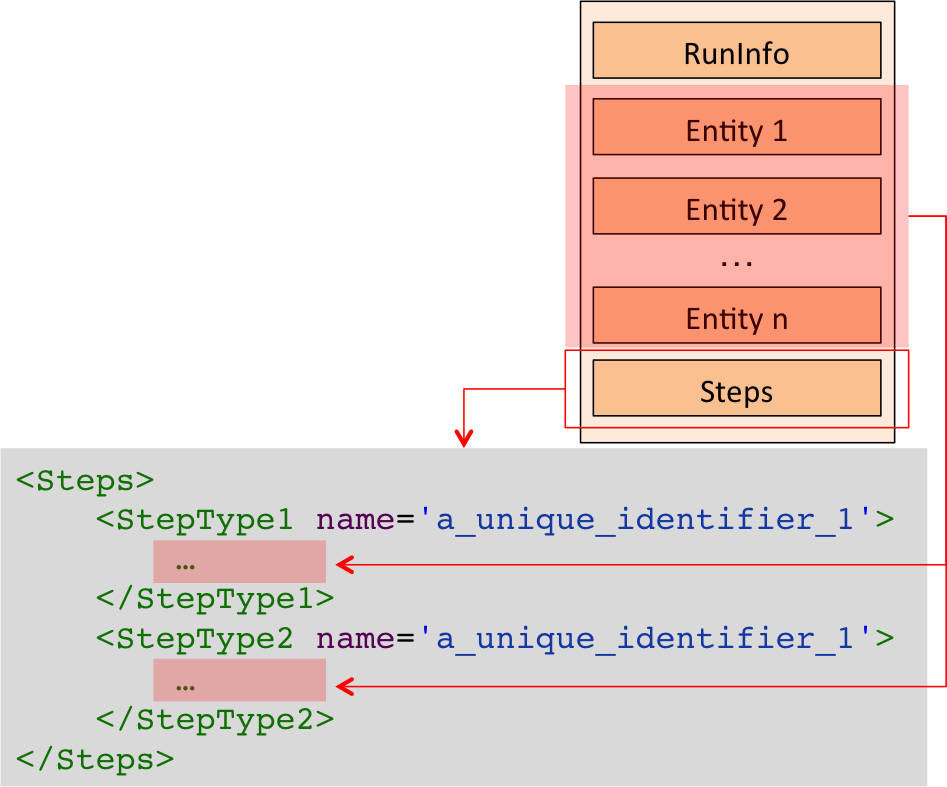
\includegraphics[scale=0.5]{pics/ExampleStepEntity.png}
  \caption{Example of the Steps \textbf{Entity}  and its connection in the input file.}
  \label{fig:ExampleStepEntity}
\end{figure}
  \item \textit{\textbf{Models}}:
  \\ The Models \textbf{Entity}  represents the projection from the input to the output space. Currently, RAVEN defines the
  following sub-categories:
      \begin{itemize}
       \item \textit{Code}, the sub-~\textbf{Entity} that represent the driven code, through external code interfaces (see~\cite{RAVENuserManual})
       \item  \textit{ExternalModel}, the sub-~\textbf{Entity} that represents a physical or mathematical model that is
       directly implemented by the user in a Python module
      \item \textit{ROM}, the sub-~\textbf{Entity} that represent the Reduced Order Model, interfaced with several algorithms
       \item \textit{PostProcessor}, the sub-~\textbf{Entity} that is used to perform action on data, such as computation of
       statistical moments, correlation matrices, etc.
      \end{itemize}
      The Model \textbf{Entity} can be seen as a transfer function between the input and output space.
  \item \textit{\textbf{Functions}}:
   \\ The Functions \textbf{Entity} is the container of all the user-defined functions, such as Goal Functions in adaptive
   sampling strategies, etc.
\end{itemize}
All these action-objects are combined together in order to create a peculiar analysis flow, which is specified
by the user in an additional \textbf{Entity} named \textit{\textbf{Steps}}. This \textbf{Entity} represents the core of the analysis, since it is the location where the multiple objects get finally linked in order to perform a combined action on a certain \textit{Model} (see Fig.~\ref{fig:ExampleStepEntity}). In order to perform this linking, each \textbf{Entity} defined in the Step needs to ``play'' a Role:
\begin{itemize}
  \item \textit{Input}
  \item \textit{Output}
  \item \textit{Model}
  \item \textit{Sampler}
  \item \textit{Function}
  \item \textit{ROM}
  \item \textit{SolutionExport}, the \textbf{Entity} that is used to export the solution of a \textit{Sampler}.
\end{itemize}
Currently, RAVEN supports 4 different types of \textit{\textbf{Steps}}:
\begin{itemize}
  \item \textit{SingleRun}, perform a single run of a model
  \item \textit{MultiRun}, perform multiple runs of a model
  \item \textit{RomTrainer}, perform the training of a Reduced Order Model (ROM)
  \item \textit{PostProcess}, post-process data or manipulate RAVEN entities
  \item \textit{IOStep}, step aimed to perform multiple actions:
  \begin{itemize}
    \item construct/update a Database from a DataObjects and vice-versa
    \item construct/update a Database or a DataObjects object from CSV files
    \item stream the content of a Database or a DataObjects out through an OutStream
    \item store/retrieve a ROM to/from an external File using Pickle module of Python
  \end{itemize}
\end{itemize}

\subsection{Raven Input Structure}
\label{sub:InputStructure}
The RAVEN code does not have a fixed calculation flow, since all of its basic
objects can be combined in order to create a user-defined calculation flow.
%
Thus, its input (XML format) is organized in different XML blocks, each with a
different functionality.
%
The main input blocks are as follows:
\begin{itemize}
  \item \xmlNode{Simulation}: The root node containing the
  entire input, all of
  the following blocks fit inside the \emph{Simulation} block.
  %
  \item \xmlNode{RunInfo}: Specifies the calculation
  settings (number of parallel simulations, etc.).
  %
  \item \xmlNode{Files}: Specifies the files to be
  used in the calculation.
  %
  \item \xmlNode{Distributions}: Defines distributions
  needed for describing parameters, etc.
  %
  \item \xmlNode{Samplers}: Sets up the strategies used for
  exploring an uncertain domain.
  %
  \item \xmlNode{DataObjects}: Specifies internal data objects
  used by RAVEN.
  %
  \item \xmlNode{Databases}: Lists the HDF5 databases used
  as input/output to a
  RAVEN run.
  %
  \item \xmlNode{OutStreams}: Visualization and
  Printing system block.
  %
  \item \xmlNode{Models}: Specifies codes, ROMs,
  post-processing analysis, etc.
  %
  \item \xmlNode{Functions}: Details interfaces to external
  user-defined functions and modules.
  %
  the user will be building and/or running.
  %
  \item \xmlNode{Steps}: Combines other blocks to detail a
  step in the RAVEN workflow including I/O and computations to be performed.
  %
\end{itemize}

Each of these blocks are explained in dedicated sections in the user manual ~\cite{RAVENuserManual}.
%
